\subsection{Einbindung für Erlang}

\begin{frame}
\begin{center}

\includegraphics[scale=0.5]{erlang/pics/erlang.png}
\end{center}
\end{frame}

\begin{frame}
  \frametitle{Generelles Einbinden einer Sprache}
  \begin{center}
    Änderung an 2 Stellen:\\$~$\\
    \includegraphics[scale=0.70]{erlang/pics/Spracheinbindung}
  \end{center}
\end{frame}

\begin{frame}
\frametitle{Piratenlogik für Erlang}
\begin{columns}
    \column[t]{0.50\textwidth}
%\begin{center}
  \includegraphics[scale=0.5]{erlang/pics/ErlangVerarbeitung}
%\end{center}
    \column[t]{0.50\textwidth}
    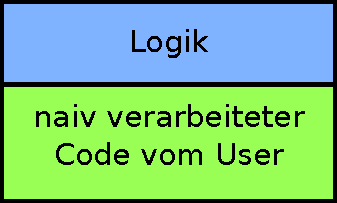
\includegraphics[scale=0.5]{erlang/pics/ErlangVerarbeitungB}
\end{columns}
wie in Ruby 
naiver ansatz 
Finde $->$ und kopiere dahinter die line function

in nächster Zeit folgt
Ziel\\
für besseres highlighting die line-Funktion mit in die vordefinierten Funktionen kopieren
funktionsvariablen verfolgen lassen\\
falsche pfeile erkennen, bzw richtige\\
Diagramm
\end{frame}

\begin{frame}
%wie bei ruby schiffslogik wird davor kopiert
%und der code entsprechend verarbeitet, \\
laufzeitfehlermeldungen ohne shell hässlich, werden abgefangen und hübsch weitergeleitet
debugging bild / zeigen
\end{frame}

\begin{frame}
\begin{center}
\LARGE Fazit
\end{center}
\end{frame}
